\documentclass[UTF8]{article}
\usepackage{ctex}
\usepackage{anyfontsize}
\usepackage{bookmark}
\usepackage{tikz}
\hypersetup{hidelinks}
\usepackage{tocbibind}
\usepackage[a4paper, top=2cm, bottom=2cm,right=2cm, left=2cm]{geometry}
\usepackage{amsmath}
\numberwithin{equation}{section}
\usepackage{mathrsfs}
\usepackage{physics}
\usepackage{booktabs}
\usepackage{bm}
\usepackage{tcolorbox}
\usepackage{amsthm}

\newtheorem*{problem}{Problem}


\usepackage{fancyhdr}
\pagestyle{fancy}
\fancyhf{} % 清空当前设置的页眉和页脚
\lhead{\leftmark} % 设置左边的页眉内容为当前子章节标题
\chead{} % 中间留空
\rhead{\thepage} % 设置右边的页眉内容为页码


\title{Notes of principles of quantum mechanics}
\author{李承高}
\begin{document}
\maketitle
\thispagestyle{empty}
\newpage
\thispagestyle{empty}
\tableofcontents
\newpage

\pagenumbering{arabic}

\section{量子力学引入}
\subsection{一些假设(postulates)}
我们在这一章节强调的是经典力学与量子力学的对应性以及区别,我们首先给出
这些假设:
\begin{enumerate}
    \item 在经典力学中,一个粒子的态可以由$x(t),p(t)$来确定,
          在量子力学中只需要一个希尔伯特空间当中的态矢量$\ket{\psi(t)}$就可以确定.
    \item 经典力学中的力学量可以用一个函数$\omega(x,p)$来描述,
          而在量子力学当中需要使用厄密算符的在某一态下的矩阵元素例如$\mel{x}{X}{x'},\mel{x}{P}{x'}$来表示.
    \item 经典力学的测量得到一个不变的状态,而量子力学的测量将会导致系统的态
          发生改变($\ket{\psi}\rightarrow \ket{\omega}$)
    \item 经典力学的状态变量随时间改变的方程遵循哈密顿方程$\dot{x}=\pdv{H}{p},
              \dot{p}=\pdv{H}{x}$,而量子力学是遵循薛定谔方程$i\hbar\dv{}{t}\ket{\psi}=H\ket{\psi}$,
          这里的哈密顿量变成量子哈密顿算符。
\end{enumerate}
叠加态原理:一个粒子可能处于的态$\ket{\psi},\ket{\psi'}$,这个态也可以写
成$\alpha\ket{\psi}+\beta\ket{\psi'}$。
\subsection{测量(measurement)}
经典力学中,$x,p$被测量,则对应的力学量$\omega(x,p)$也能够被获得,而在量子力学中,
\begin{tcolorbox}[colframe=red,title=量子力学中的测量步骤]
    \begin{enumerate}
        \item 构造出对应的力学量算符$X,\Omega$
        \item 计算算符本征值和正交本征态
        \item 将$\ket{\psi}$在其本征矢上展开得到$\ket{\psi}=\sum_i\ket{\omega_i}\braket{\omega_i}{\psi}$
    \end{enumerate}
\end{tcolorbox}
这样我们可以定义在$\ket{\omega}$基上测量得到$\omega_i$的概率$P(\omega_i)$正比于$\abs{\braket{\psi}{\omega_i}\braket{\omega_i}{\psi}}^2$也就是$\abs{\psi(\omega_i)}^2$
量子力学可以预测$\Omega$的可能测量结果的概率值,$\Omega$在其本征态上测量结果只能是它的这些本征值。

\begin{tcolorbox}[
    colframe = blue,
    title = 相对概率和绝对概率的区别
]
   没有归一化的的态得到的概率是相对概率,归一化之后的是绝对概率 
\end{tcolorbox}
\noindent \textbf{总结:如果存在一个在希尔伯特空间的态$\ket{\psi}$,那么其包含了所有
观测量的信息}

在已经得到$\ket{\psi}$在基$\ket{\omega}$下的信息,想要得到基
$\ket{\lambda}$下的信息,并不需要每次都重新测量测量,基变换推导(通过插入封闭
关系式,也可以称之为投影算符):
\begin{align*}
    \ket{\omega} = \sum_i \ket{\lambda}\bra{\lambda}\ket{\omega}
\end{align*}

态矢坍塌(collapse)的定义:在测量之前,态矢可以写成某些基矢下的线性叠加:
\begin{align*}
    \ket{\psi}=\sum_\omega \ket{\omega}\braket{\omega}{\psi}
\end{align*}
\noindent 在测量的本征值为$\omega$之后,我们进入了$\ket{\omega}$,这样的过程就是
态矢坍塌了。

\begin{tcolorbox}[
    opacityback = 1
]
    \begin{problem}
    如何检测量子理论?
    \end{problem}
量子理论的测量是要告诉我们测量之后的信息而非测量之前的,我们需要测量概率
必须重复很多次实验,但是我们不能对一个粒子进行重复实验在量子理论当中
,因此我们使用包含了N个处于$\ket{\omega}$粒子量子系综,当粒子数足够多
的时候,在测量之后,得到的处于某一态的粒子数的偏差是很小的。
\end{tcolorbox}


两个描述量子系综的统计量:期望和方差
\begin{align*}
     & \expval{\Omega}=\sum_i \omega_i P(\omega_i)=\sum_i \abs{\braket{\omega_i}{\psi}}^2\omega_i
    =\sum_i\mel{\psi}{\Omega}{\omega_i}\braket{\omega_i}{\psi}=\mel{\psi}{\Omega}{\psi}           \\
     & (\Delta \Omega)^2=\sum_i P(\omega_i)(\omega_i-\expval{\Omega})^2
    =\mel{\psi}{(\Omega-\expval{\Omega})^2}{\psi}
\end{align*}
没有两个单独的测量可以同时进行,如果$\expval{X}=a,\Delta X=\Delta$,我们
可以理解为粒子很可能在位置为a的地方发现,其偏差为$\Delta$。
\subsection{泊松括号和对易关系}
在经典力学中,两个力学量是否对易使用泊松括号来描述的:
\begin{align*}
    {A,B} = \pdv{A}{q}\pdv{B}{p}-\pdv{A}{p}\pdv{B}{q}
\end{align*}
其中p和q为广义坐标和广义动量,在量子力学中使用力学量算符的对易关系来描述:
\begin{align*}
    [A,B] = AB-BA
\end{align*}
量子力学中,两个算符是否具有共同本征态可以使用对易关系是否为0来判断。常用的一些
关于对易关系的计算:
\begin{align*}
    [AB,C] = A[B,C]+[A,C]B
\end{align*}
\subsection{薛定谔方程的引入}
假设H在这里不显含时间:
\begin{align*}
    i\hbar \dot{\ket{\psi}}=H\ket{\psi}
\end{align*}
利用定态薛定谔方程:$H\ket{E}=E\ket{E}$,将态在能量基上展开,得到:
\begin{align*}
    \ket{\psi}=\sum_E
    \ket{E}\braket{E}{\psi(t)}=\sum_E a_E (t)\ket{E}
\end{align*}
利用含时薛定谔方程,两边作用于
$i\hbar \partial/ \partial t-H$得到:
\begin{align*}
     & i\hbar \dot{a}_E(t)=Ea_E(t)                                 \\
     & a_E(t)=a(0)e^{-iEt/\hbar}=\braket{E}{\psi(0)}e^{-iEt/\hbar} 
\end{align*}
因此,含时态可以看成能量本征函数的线性组合:
\begin{tcolorbox}[colframe=red]
    $$\ket{\psi(t)}=\sum_E \ket{E}\bra{E}e^{-iEt/\hbar}\ket{\psi(0)}$$
\end{tcolorbox}
\noindent 可以在能量本征态上定义传播子:
\begin{align*}
    U(t) = \sum_E \ket{E}\bra{E}e^{-iEt/\hbar}
\end{align*}
更一般的情况:
\begin{align*}
    U(t)=e^{-iHt/\hbar}
\end{align*}

在求解薛定谔方程时,通常根据问题来选择不同的基,例如对于
恒力产生的势场,我们更偏向于选择动量本征函数作为基,对于V很复杂的情况
选择坐标本征函数作为基。
\section{一维定态问题}
\subsection{定态和束缚态的定义}
定态是量子力学中一个非常重要的概念,引入:如果定态也是含时的,则根据上一节的公式:
\begin{tcolorbox}[
    colframe = red,
    title = 定态的定义
]
    \begin{equation*}
        \ket{E(t)} = \sum_E \ket{E(0)}e^{-iEt/\hbar}
    \end{equation*}
\end{tcolorbox}
处于定态的系统有以下性质:
\begin{enumerate}
    \item 概率密度不随时间变化
    \item 力学量算符平均值不随时间变化
    \item 概率流密度不随时间变化
\end{enumerate}

\begin{tcolorbox}[colframe=green,title = 束缚态的定义]
    当系统的$E<V$时,系统处于束缚态,处于束缚态的系统的
    能量
是离散的,因为在无穷远处,波函数为0.
\end{tcolorbox}

\subsection{自由粒子}
自由粒子的定态薛定谔方程:
\begin{align*}
    \frac{P^2}{2m}\ket{E}=E\ket{E}
\end{align*}
将薛定谔方程放在p的本征态组成的线性空间(简称p空间)中进行求解,在这个线性空间中,p是定值
\begin{align*}
    \frac{P^2}{2m}\ket{p}=E\ket{p}
\end{align*}
得到的本征函数:$\ket{\sqrt{2mE}}$和$\ket{-\sqrt{2mE}}$,本征能量为$P^2/2m$。是二重
简并的。
\subsection{势阱中的粒子}
势阱中的粒子,经典力学中的束缚态,就是把粒子束缚在井内,量子力学中的束缚态
导致了能量本征值变成离散的,波函数在无穷远处趋近于0,并且和经典情况描述的类似:$
    V(\pm \infty)>E$。

讲到这里就要提一下边界条件了:如果$V(x)$是有限的,则波函数和波函数的倒数均在此连续
否则只是波函数在此连续。我们这里解一个一维无限深势井:
\begin{align*}
    V(x)=\begin{cases}
             0      & \abs{x}<\frac{L}{2} \\
             \infty & \abs{x}>\frac{L}{2}
         \end{cases}
\end{align*}
\begin{align*}
     & (\frac{P^2}{2m}+V(x))\psi(x)=E\psi(x)                       \\
     & \frac{d^2}{dx^2}\psi(x)+\frac{2m}{\hbar^2}(E-V(x))\psi(x)=0
\end{align*}
这里由势能分成的三个区域分别由三个波函数:$\psi_1(x),\psi_2(x),\psi_3(x)$,可以得到
边界条件:
\begin{align*}
     & \psi_1(-\frac{L}{2})=\psi_2(-\frac{L}{2}) \\
     & \psi_2(\frac{L}{2})=\psi_3(\frac{L}{2})
\end{align*}
对于一区域和三区域,当$V(x)=\infty$时,$\psi = 0$,但对于二区域:
\begin{align*}
    \frac{d^2\psi(x)}{dx^2}+\frac{2m}{\hbar^2}E\psi(x)=0\Rightarrow \psi(x)=
    Ae^{i\alpha x}+Be^{-i\alpha x}(\alpha = \sqrt{\frac{2mE}{\hbar^2}})
\end{align*}
代入边界条件:
\begin{align*}
    \begin{cases}
        e^{i\alpha \frac{L}{2}}A+e^{-\alpha\frac{L}{2}}B=0 \\
        e^{-i\alpha \frac{L}{2}}A+e^{i\alpha \frac{L}{2}}B=0
    \end{cases}
    \Rightarrow
    \mqty[e^{i\alpha\frac{L}{2}} & e^{-i\alpha \frac{L}{2}}       \\
    e^{-i\alpha\frac{L}{2}}      & e^{i\alpha\frac{L}{2}}]\mqty[A \\B]=0
\end{align*}
可以得到:
\begin{align*}
    \alpha =\frac{n\pi}{L},E=\frac{n^2\pi^2\hbar^2}{2mL^2}
\end{align*}
其本征波函数:
\begin{align*}
    Ae^{i\alpha L}=-B \\
    \psi(x)=Ae^{i\alpha x}-Ae^{i\alpha L}e^{-i\alpha x}
\end{align*}
归一化的问题一定是模方积分等于1,而不是直接积分,千万要注意:
\begin{align*}
    \psi(x)=\begin{cases}
                C\sin \alpha x \qquad n\quad even \\
                C'\cos \alpha x \qquad n \quad odd
            \end{cases}
\end{align*}
得到归一化后的波函数:
\begin{align*}
    \psi(x)=\begin{cases}
                \sqrt{\frac{2}{L}} \sin \frac{n\pi}{L} \\
                \sqrt{\frac{2}{L}} \cos \frac{n\pi}{L}
            \end{cases}
\end{align*}
关于束缚态的一些结论:对于束缚态的能级是离散的,对于V是有限的情况,我们满足的连续
性条件除了要求波函数在边界处是连续的,波函数的导数在边界处也是连续的。
\subsection{连续性方程}
连续性方程在电磁学当中的定义:
\begin{align*}
    \frac{\partial \rho}{\partial t}+\nabla \cdot j=0
\end{align*}
现在我们把$\rho$看成概率密度,而j看成流密度,这样我们根据含时薛定谔方程:
\begin{align*}
    i\hbar \pdv{\psi}{t}&=(-\frac{\hbar^2}{2m}\nabla^2+V)\psi  &(1) \\
    -i\hbar \pdv{\psi^*}{t}&=(-\frac{\hbar^2}{2m}\nabla^2+V)\psi^* &(2)
\end{align*}
由$(1)*\psi^*-(2)*\psi:$
\begin{align*}
    i\hbar\pdv{P}{t}= & \frac{\hbar^2}{2m}(\psi^*\nabla^2 \psi-\psi\nabla^2 \psi^*)     \\
    =                 & \frac{i\hbar}{2m}\nabla\cdot(\psi\nabla\psi^*-\psi^*\nabla\psi)
\end{align*}
与连续性方程进行对比可以发现:
\begin{align*}
    j=\frac{i\hbar}{2m}(\psi\nabla\psi^*-\psi^*\nabla\psi)
\end{align*}
\subsection{散射问题}
考虑两类情况,一类是粒子的能量小于势垒的势能,在经典力学中粒子一定会被反射
回来,但是在量子力学中有一定几率穿过势垒,这种现象被称为量子隧穿效应,还有
一种情况就是当粒子能量大于势阱的势能时,经典力学中是一定穿过,但是在量子力学
中有一定的几率返回。

这类散射问题中一般要求我们求出透射系数T和反射系数R\newline
此处给出一个求上述两个系数例子:现在有一个粒子$E>V_0$,其中$V_0$作用的范围为$0<x<a$,求此时透射系数和反射系数。\newline
根据定态薛定谔方程的解可以得到以下不同区域的粒子的波函数:
$$
    \begin{array}{l}
        \psi _1=e^{ikx}+Ae^{-ikx}              \\
        \psi _2=Be^{i\alpha x}+Ce^{-i\alpha x} \\
        \psi _3=De^{ikx}                       \\
    \end{array}
$$
其中$R=|A|^2,T = |D|^2$,结合边界条件和连续性条件,可以获得这两个系数。

\section{量子谐振子}
\subsection{X basis}
量子谐振子所满足的薛定谔方程:
\begin{align*}
    (\frac{P^2}{2m}+\frac{1}{2}m\omega^2x^2)\Psi(x)=E\Psi(x)
\end{align*}
对应的解为:
\begin{align*}
    \Psi(x) = Ae^{-\alpha^2 x^2 /2}H_n(\alpha x)\quad \alpha = \sqrt{\frac{m\omega}{\hbar}}
\end{align*}
其中$H_n(\alpha x)$为厄密多项式,可以使用以下递推关系式来推导:
\begin{align*}
    H_n(x) = (-1)^n e^{x^2}\frac{d^n}{dx^n}(e^{-x^2})
\end{align*}
根据递推关系式得出前几项的厄密多项式:
\begin{align*}
    &H_0(x) = 1\\
    &H_1(x) = 2x\\
    &H_2(x) = 4x^2-2\\
    &\cdots
\end{align*}
对于$A_n$,就是归一化常数,使用的时候进行归一化就行了,一般是对前几个能级进行归一化并不是
很复杂。此外这里的厄密多项式还有一个特点,就是当n为偶数时,厄密多项式为偶函数,当n为奇数时,
厄密多项式为奇函数,这里的结论在讨论对称性时是很有帮助的。
\subsection{E basis}
考虑到粒子占有数算符:
\begin{align*}
    N \ket{n} = n \ket{n} \quad N = a^\dagger a
\end{align*}
通过
\begin{align*}
    \frac{H}{\hbar\omega}&=\frac{m\omega}{2\hbar}X^2+\frac{1}{2m\hbar\omega}P^2\\
                         &=\left(\sqrt{\frac{m\omega}{2\hbar}}X-i\sqrt{\frac{1}{2m\hbar\omega}}P\right)
                         \left(\sqrt{\frac{m\omega}{2\hbar}}X+i\sqrt{\frac{1}{2m\hbar\omega}}P\right)+c
\end{align*}
可以构造两个算符:
\begin{align*}
    a         & = \sqrt{\frac{m\omega}{2\hbar}}X+i\sqrt{\frac{1}{2m\omega\hbar}}P \\
    a^\dagger & = \sqrt{\frac{m\omega}{2\hbar}}X-i\sqrt{\frac{1}{2m\omega\hbar}}P 
\end{align*}
并且得到对易关系:
\begin{align*}
    &[a,a^\dagger]=1                                                    \\
    &[a,\hat{H} ]=[a,aa^\dagger]=a[a,a^\dagger]=a
\end{align*}
这两个算符正是粒子数的产生和湮灭算符,并且这两个算符满足以下
递推关系:
\begin{tcolorbox}[
    colframe=red,
]
\begin{equation*}
    \begin{aligned}
    a^\dagger\ket{n} &= \sqrt{n+1}\ket{n+1}\\
    a\ket{n} &= \sqrt{n}\ket{n-1}\quad \\
    a\ket{0} &= 0
    \end{aligned}
\end{equation*}
\end{tcolorbox}
\subsection{从E basis到X basis}
首先使用产生算符使粒子数从0变为n:
\begin{align*}
    (a^\dagger\ket{0})^n = \sqrt{n!} \ket{n} 
\end{align*}
从E basis变换到X basis
\begin{align*}
     & (a^\dagger)^n\braket{x}{\psi_0}=\sqrt[]{n!}\braket{x}{\psi_n} \\
\end{align*}
此时的$a^\dagger$是在X表象中表示的:
\begin{align*}
     & a^\dagger = \sqrt{\frac{m\omega}{2\hbar}}x-\sqrt{\frac{\hbar}{2m\omega}}\frac{d}{dx}                         \\
     & y = \sqrt{\frac{m\omega}{\hbar}}x\Rightarrow a^\dagger = \frac{1}{\sqrt{2}}
    (y-\frac{d}{dy})                                                        \\
     & \psi_n(x)=\frac{1}{\sqrt{n!}}\frac{1}{(\sqrt{2})^n}(y-\frac{d}{dy})^n(\frac{m\omega}{\pi \hbar})^\frac{1}{4}
    e^{-y^2/2}
\end{align*}
\section{多粒子系统}
\subsection{直积运算}
在这里稍微区分一下基矢和态,现在考虑到两粒子系统:
$\ket{x_1}\bigotimes\ket{x_2}\rightarrow \ket{x_1x_2}$,还有直积,内积,外积的区别:
$\braket{\psi_1}{\psi_2},\ket{\psi_1}\bra{\psi_2}$,这两个矢量是属于同一个希尔伯特空间
的,对于直积,两个矢量属于不同的希尔伯特空间。线性无关的基矢数目对应的维数,$m\bigotimes
    n\rightarrow m\times n$dim,$ m\bigoplus n \rightarrow m+n $dim。

态矢直积归一化:
\begin{align*}
    (\bra{x_1'}\bigotimes\bra{x_2})(\ket{x_1}\bigotimes \ket{x_2})=\delta(x_1'-x_1)\delta(x_2'-x_2)
\end{align*}

算符直积作用于态矢:
\begin{align*}
    X_1^{(1)\bigotimes(2)}(\ket{x_1}\bigotimes\ket{x_2})=x_1\ket{x_1}\bigotimes I_2^{(2)}\ket{x_2}
\end{align*}
\subsection{两粒子态矢的演化}
定态薛定谔方程:
\begin{align*}
    (H_1+H_2+V(x_1,x_2))\ket{E_1}\bigotimes\ket{E_2}=(E_1+E_2)\ket{E_1}\bigotimes\ket{E_2}
\end{align*}

case A:$V(x_1,x_2)=V(x_1)+V(X_2)$,此时可以直接分离变量,考虑到在坐标基矢中:
\begin{align*}
    \frac{1}{\psi_{E_1}(x)}H_1\psi_{E_1}(x)=\frac{1}{\psi_{E_2}}H_2\psi_{E_2}=E_1+E_2
\end{align*}
然后得到两个定态薛定谔方程。这样情况A就解决了。

Case B:$V(x_1,x_2)=V(x_1-x_2)$,此时我们采用在质心系当中解决两体问题的方法来解决
这种类型的问题:\\
先考虑经典力学中:
\begin{align*}
     & F_{12}=m_1a_1,F_{21}=m_2a_2,F_{12}=-F_{21}         \\
     & a_1-a_2 = -\frac{m_1+m_2}{m_1m_2}F_{21}            \\
     & a_r = \frac{F_r}{\mu},\mu = \frac{m_1m_2}{m_1+m_2}
\end{align*}
在量子力学情形中:
\begin{align*}
     & V(x_1,x_2)=V(x_1-x_2),x_{cm}=\frac{m_1x_1+m_2x_2}{m_1+m_2},x_r=x_1-x_2                               \\
     & (\frac{P_{cm}^2}{2M}+\frac{p^2}{2\mu}+V(x_r))\psi_{cm}(r)\psi_r(r)=(E_{cm}+E_r)\psi_{cm}(r)\psi_r(r)
\end{align*}
由于cm项类似于自由粒子的哈密顿量,因此此时可以和右边的能量本征值消掉,因此就得到了两粒子
体系态矢随演化的方程:
\begin{align*}
    (\frac{p_r^2}{2\mu}+V(x_r))\psi_r(r)=E_r\psi_r(r)
\end{align*}
\subsection{全同粒子}
交换位置后,系统的态矢量不变可以视为两粒子不可区分,数学推导:
\begin{align*}
    \beta \ket{ab}+\gamma\ket{ba}=\alpha(\beta \ket{ba}+\gamma\ket{ab}) \\
    \begin{cases}
        \gamma = \alpha\beta \\
        \beta = \alpha\gamma
    \end{cases}\Rightarrow \alpha = \pm 1,\beta = \pm \gamma
\end{align*}
$\alpha =1$对应的是对称,$\alpha = -1$对应的是反对称,根据对称性的不同,我们可以定义
出玻色子和费米子,满足对称性的是玻色子,满足反对称性的是费米子,举例子:pi介子,光子
引力子属于玻色子,电子中子质子属于费米子,满足泡利不相容原理,即$a\neq b$,文字
描述就是两个或两个以上的费米子不能处于相同的态上。

QFT中的自旋统计理论:自旋是$\frac{\hbar}{2}$的偶数倍是玻色子,自旋是$\frac{\hbar}{2}$的
奇数倍是费米子,这个理论仅适用于三维情况。如果是一维情况则根据对称性来判断。

在原子核,原子,分子等复合粒子中,凡是由玻色子构成的复合粒子是波色子,由偶数个费米子构成的也为波色子;由奇数个费米子构成的系统称为费米子。

两粒子体系的希尔伯特空间可以由玻色和费米矢量的希尔伯特空间组成:
\begin{align*}
    V_{1\bigotimes 2}=V_A\bigoplus V_S
\end{align*}
其中由于泡利不相容原理使得$dim V_S>dim V_A$。
\subsection{全同粒子态矢归一化}
对于离散情况:
\begin{align*}
     & \ket{\omega_1\omega_2,S}=\frac{1}{\sqrt{2}}(\ket{\omega_1\omega_2}+\ket{\omega_2\omega_1}) \\
     & P_S(\omega_1\omega_2)=|\braket{\omega_1\omega_2,S}{\psi}|^2                                \\
     & \sum_{\omega_1=min}\sum_{\omega_2=min}P_S(\omega_1\omega_2)=1
\end{align*}
由于对于每个$\omega$都加了两次,因此最终的结果需要除以2。

对于连续的情况:
\begin{align*}
     & \ket{\omega_1\omega_2,S}=\frac{1}{\sqrt{2}}(\ket{\omega_1\omega_2}+\ket{\omega_2\omega_1}) \\
     & 1=\iint |\braket{\omega_1\omega_2,S}{\psi}|^2 \frac{d\omega_1d\omega_2}{2}                 \\
     & \psi_S(\omega_1\omega_2)=\frac{1}{\sqrt{2}}\braket{\omega_1\omega_2,S}{\psi}               \\
     & P_S(\omega_1\omega_2)=|\braket{\omega_1\omega_2,S}{\psi}|^2=2|\psi_S(\omega_1\omega_2)|^2
\end{align*}
只有在连续情况下才能定义波函数,P的定义为了统一应与离散情况下一致,所以满足此要求,那波函数就需要另外
定义。

N个费米子组成的系统的波函数由slater行列式构成:
\begin{align*}
    \psi(x_1,x_2\cdots,x_N)=\frac{1}{\sqrt{N!}}\mdet{\psi_1(x_1) & \psi_1(x_2) & \cdots & \psi_1(x_N) \\\psi_2(x_1)&\psi_2(x_2)&\cdots&\psi_2(x_N)\\
                                                                 &             & \cdots &             \\ \psi_N(x_1)&\psi_N(x_2)&\cdots&\psi_N(x_N)}
\end{align*}
\subsection{可以忽略对称性与反对称性的情况}
如果两个粒子的态几乎没有发生交叠,可以忽略对称性与反对称性的情况。

这里举一个例子:
设想一个pion的在地球上,并且处于基态,另外一个pion在月球上,在地球上的到的波函数
$\psi_E(x_E)$,在月球上得到了波函数$\psi_M(x_M)$,现在考虑到对称性:
\begin{align*}
    \psi_S(x_E,x_M)=\frac{1}{\sqrt{2}}(\psi_E(x_E)\psi_M(x_M)+\psi_E(x_M)\psi_M(x_E))
\end{align*}
因此由一节连续情况的全同粒子态矢与波函数的关系得到:
\begin{align*}
    P_S(x_E,x_M) & =2|\psi_S(x_Ex_M)|^2=|\psi_E(x_E)\psi_M(x_M)+\psi_E(x_M)\psi_M(x_E)|^2                    \\
                 & =|\psi_E(x_E)|^2|\psi_M(x_M)|^2+|\psi_E(x_M)|^2|\psi_M(x_E)|^2+\psi^*_E(x_E)\psi^*_M(x_M)
    \psi_E(x_M)\psi_M(x_E)+\text{共轭项}
\end{align*}
对Moon项积分:
\begin{align*}
    P_S(x_E) & =\int 2|\psi_S(x_Ex_M)|^2 dx_M=\int|\psi_E(x_E)\psi_M(x_M)+\psi_M(x_E) \psi_E(x_M)|^2dx_M \\
             & =|\psi_E(x_E)|^2\int|\psi_M(x_M)|^2dx_M+|\psi_M(x_E)|^2\int|\psi_E(x_M)|^2dx_M            \\
             & +\psi^*_E(x_E)\psi_M(x_E)\int \psi^*_M(x_M)
    \psi_E(x_M)dx_M+\text{共轭项}
\end{align*}
如果两个粒子的波函数并没有交叠$\psi_M(x_E),\psi_E(x_M)$都很小,因此:
\begin{align*}
    P_S(x_E)=|\psi_E(x_E)|^2
\end{align*}
反之对Earth积分,会得到类似的结果:
\begin{align*}
    P_S(x_M)=|\psi_M(x_M)|^2
\end{align*}
\section{对称性与守恒量}
对称性与守恒量的关系是基于Enrenfest-Theorem:
\begin{align*}
    \frac{d\expval{A}}{dt}=\expval{[A,H]}+\pdv{\expval{A}}{t}
\end{align*}
一般我们研究的力学量算符在不显含时间时,可以忽略掉偏导项,这样力学量算符的
守恒关系可以简化为:
\begin{align*}
    \expval{[A,H]}=0
\end{align*}
则当A和H对易时,A是守恒量。注释:诺特定理:每个连续对称性和一个守恒量
一一对应。
\subsection{空间平移对称性}
在经典力学中,平移对称性蕴含在这两个式子中:
\begin{align*}
    x_{\varepsilon}\rightarrow x+\varepsilon \\
    p_{\varepsilon}=p
\end{align*}
由于在量子力学当中,位置和动量不能够被同时测量,但是平均值是能够被测量的,我们使用平均值是量子力学能够与经典力学对应。
量子力学中的平移由这两个式子定义:
\begin{align*}
    \expval{X_{\varepsilon}}\rightarrow \expval{X}+\varepsilon \\
    \expval{P_{\varepsilon}}=\expval{P}
\end{align*}
到这里我们有两种角度去描述平移,一种是态的角度,一种是算符的角度,分别对应的是主动的变换和被动的变换。

\textbf{主动观点}:
\begin{align*}
    \expval{X}{\psi_{\varepsilon}}=\expval{X}{\psi}+\varepsilon \\
    \ket{\psi_{\varepsilon}}=T(\varepsilon)\ket{\psi}
\end{align*}

\textbf{被动观点}:
\begin{align*}
    X_{\varepsilon}=T^\dagger(\varepsilon)XT(\varepsilon)
\end{align*}

现在主要来研究主动的观点:
在x basis通过波函数来研究态的平移行为:
\begin{align*}
    \matrixel{x}{T(\varepsilon)}{\psi}=\psi(x-\varepsilon)
\end{align*}
分别对算符和波函数展开,这里展开到一阶项,研究无穷小的平移:
\begin{align*}
    \matrixel{x}{I-\frac{ip}{\hbar}\varepsilon}{\psi}=\psi(x)+\frac{d\psi(x)}{dx}(-\varepsilon)
\end{align*}
我们可以得到平移算符的表达式:
\begin{align*}
    T(\varepsilon)=e^{-ip\varepsilon/\hbar}
\end{align*}
对于有限小的平移也是这样的,我们可以考虑一个有限小平移a,将其分成N份,N趋近于
无穷大,这样就可以通过将有限小平移分解成无限小平移进行处理,进行N次平移:
\begin{align*}
    \lim_{N\rightarrow \infty} (I-\frac{ip}{\hbar}\frac{a}{N})^N=e^{-\frac{ip a}{\hbar}}
\end{align*}
可以得到有限平移算符。
动量守恒是由于空间的平移不变性导致的。
\begin{align*}
    \expval{H}{\psi_{\varepsilon}}=\expval{H}{\psi}\Rightarrow [P,H]=0
\end{align*}
根据Enrenfest Theorem可以得到动量守恒:
\begin{align*}
    \frac{d\expval{P}}{dt}=0
\end{align*}
\subsection{时间平移对称性}
传播子的定义:$U(t)=e^{-iHt/\hbar}$,因此时间平移算符定义为传播子。这样我们还是
考虑到无限小时间平移,将算符展开到一阶项,根据Enrenfest-Theorem可以得到能量守恒定律:
\begin{align*}
    \frac{d\expval{H}}{dt}=0
\end{align*}
\subsection{宇称}
宇称算符定义:
\begin{align*}
    \Pi \ket{x}=\ket{-x}
\end{align*}
计算宇称算符的本征值:
\begin{align*}
    \Pi^2 \ket{x}=\ket{-(-x)}\Rightarrow \lambda = \pm 1
\end{align*}
本征值为$\pm 1$,分别对应奇宇称和偶宇称,现在使用主动的观点:
\begin{align*}
    \Pi^\dagger X \Pi = -X \\
    \Pi^\dagger P\Pi = -P
\end{align*}
如果H在宇称变换下是不变的:$\Pi\dagger H\Pi =H\Rightarrow [\Pi,H]=0$。

在时空平移和旋转不会导致自然法则的改变,但是宇称不是,在弱相互作用力下,宇称是
不守恒的。在涉及到弱相互作用力时,$[\Pi,H]\neq 0$。文字描述就是,初始状态下,如果两个态是
互为镜像,但是末态就不是互为镜像了,这样就叫做宇称不守恒了。
\subsection{时间反演对称性*}
时间反演就像是电影的倒放一样,在经典力学中的定义:
\begin{align*}
    x_r(t)\stackrel{-t}{\longrightarrow} x(t)\qquad p_r(t)\rightarrow -p(t)
\end{align*}
可以使用如下文字来描述:设想一个星球做轨道运动,在前T时间内,这个星球做逆时针
运动,在2T时刻,星球回到了初始点,位置不发生改变,但是动量的方向发生改变了,这个
是符合牛顿第二定律的。

在量子力学中的时间反演:类比于经典力学,只是这里的力学量变成了力学量算符,我们可以使用平均值来描述:
\begin{align*}
    \expval{x_r(t)}\stackrel{-t}{\longrightarrow} \expval{x(t)}\qquad \expval{p_r(t)}\rightarrow \expval{-p(t)}
\end{align*}
量子力学中的时间反演就是把态变换到其对偶项即$\psi(x)\rightarrow \psi^*(x)$,是正好满足以上关系的。
\subsection{旋转对称性}
先复习一下经典力学当中的二维旋转操作:
\begin{align*}
    \begin{cases}
        x'=r\cos{\theta+\phi} \\
        y'=r\sin{\theta+\phi}
    \end{cases}
    \Rightarrow
    \begin{cases}
        x'=x\cos{\theta}-y\sin{\theta} \\
        y'=x\sin{\theta}+y\cos{\theta}
    \end{cases}
\end{align*}
写成矩阵形式:
\begin{align*}
    \mqty[x' \\y']=\mqty[\cos{\theta}&-\sin{\theta}\\ \sin{\theta}&\cos\theta]\mqty[x\\y]
\end{align*}
考虑到无限小转动:
\begin{align*}
    \begin{cases}
        x'=x-y\theta \\
        y'=x\theta+y
    \end{cases}
\end{align*}
与无限小平移进行对比,定义绕z轴无限小转动生成元:
\begin{align*}
    U(R)=I-\frac{iL_z\theta}{\hbar}
\end{align*}
这里有两种变换,主动变换和被动变换,两者是可以互相推导出来的,先使用主动变换即
态变换,如果我们将其投影到x basis上,可以得到角动量算符在量子力学中的具体表达形式,当然这里也可以使用$r\times P$写成
分量形式来得到结果:
\begin{align*}
    \bra{xy}U(R)\ket{\psi}=\psi(x+y\theta,y-x\theta)
\end{align*}
对右边进行二元函数泰勒展开:
\begin{align*}
    \matrixel{xy}{I-\frac{iL_z \theta}{\hbar}}{\psi}=\psi(x,y)+\pdv{\psi}{x} y\theta-\pdv{\psi}{y}x\theta+o \\
    L_z = xP_y-yP_x
\end{align*}
在这里使用被动变换即算符变换。
我们现在证明H在无限小转动时如果保持H不变,我们会得到z方向角动量守恒定律:
\begin{align*}
    U^\dagger(R)HU(R)=H\Rightarrow [L_z,H]=0
\end{align*}
根据Enrenfest-Theorem得到z方向上的角动量守恒:
\begin{align*}
    \frac{d\expval{L_z}}{dt}=0
\end{align*}
有限转动类似于有限平移的推导:
\begin{align*}
    \lim_{N\rightarrow\infty}(1-\frac{iL_z\theta}{\hbar N})^N=e^{-iL_z \theta/\hbar}
\end{align*}

\section{自旋以及自旋耦合}
\subsection{自旋}
自旋是粒子的内部的角动量,一个重要的点是,角动量可以随着外部场强的改变而改变
,但是自旋是不会改变的,现在我们研究的是电子的自旋,电子的自旋大小一直是$\frac{\hbar}{2}$,
但是如果其投影在某一个具体的方向之后就有了正负代表自旋的正负。
现在引入自旋算符,这个是在$S_z$basis下定义的,其他basis可以表示为$S_z$basis的线性组合。
\begin{align*}
    S_x=\frac{\hbar}{2}\mqty[0 & 1 \\1&0],S_y=\frac{\hbar}{2}\mqty[0&-i\\i&0],S_z=\frac{\hbar}{2}\mqty[1&0\\0&-1]
\end{align*}
我们可以将其推广到任意方向,
\begin{align*}
    \begin{cases}
        n_z=\cos \theta           \\
        n_x=\sin \theta \sin \phi \\
        n_y=\sin \theta \cos\phi
    \end{cases}
\end{align*}
因此可以得到$\vu{n} \cdot S=n_xS_x+n_yS_y+n_zS_z$,在求得其本征值与本征态:
\begin{align*}
    \frac{\hbar}{2}\mqty|\cos \theta-\lambda & \sin \theta e^{-i\phi} \\ \sin\theta e^{i\phi}&-\cos \theta-\lambda|=0
\end{align*}
$\lambda=\pm 1$,因此类似与上面在$S_Z$的自身本征态下,有所谓的自旋向上和自旋向下
,接下来引入泡利矩阵就是上面的自旋算符/$\frac{\hbar}{2}$:
\begin{align*}
    \sigma_x=\mqty[0 & 1 \\1&0],\sigma_y=\mqty[0&-i\\i&0],\sigma_z=\mqty[1&0\\0&-1]
\end{align*}
泡利矩阵的一些性质,其中最重要的就是对易关系和反对易关系:
\begin{align*}
    [\sigma_i,\sigma_j]=2i\varepsilon_{ijk}\sigma_k \\
    \{\sigma_i,\sigma_j\}=2I\delta_{ij}
\end{align*}
证明:
\begin{align*}
    [S_i,S_j]=i\hbar \varepsilon_{ijk} S_k \\
    (\frac{\hbar}{2})^2[\sigma_i,\sigma_j]=i\hbar \varepsilon_{ijk} \frac{\hbar}{2}\sigma_k
\end{align*}

爱因斯坦求和约定需要注意的几个点:重复指标代表求和,对于矢量积的运算:
\begin{align*}
     & A\times B = a_i\vu{e_i}\times b_j \vu{e_j}=a_ib_j(\vu{e_i}\times\vu{e_j})=a_ib_j\varepsilon_{ijk}\vu{e_k}=\varepsilon_{ijk}a_ib_j\vu{e_k}
    \\  &a_ib_j\delta_{ij}=a_ib_i
\end{align*}
利用爱因斯坦求和约定证明:$(A\cdot\sigma)(B\cdot \sigma)=A\cdot B I+i(A\times B)\cdot \sigma$:
\begin{align*}
    a_i\sigma_i b_j\sigma_j & =a_ib_j\sigma_i\sigma_j=a_ib_j(i\varepsilon_{ijk}\sigma_k+I\delta_{ij}) \\
                            & =i\varepsilon_{ijk}a_ib_j\sigma_k+a_ib_j+a_ib_i I                       \\
                            & =A\cdot B I+i(A\times B)\cdot \sigma
\end{align*}
上面都是介绍的与自旋相关的算符,现在我们来介绍和自旋有关的态:(假设都是处于$S_z$的本征态)
在考虑自旋时,我们需要考虑额外的自由度,考虑到直积(derect product):$
    V_o\bigotimes V_s$,spinor描述一个有两个自旋方向的波函数:
\begin{align*}
    \mqty[\psi_+ \\ \psi_-]=\psi_+ \mqty[1\\0]+\psi_- \mqty[0\\1]
\end{align*}
在Hilbert空间中,开始是$\infty$维的,但是现在引入自旋之后变成$2\infty$维了。
\subsection{自旋耦合}
两个粒子的自旋耦合可以写成:$\ket{s_1m_1,s_2m_2}=\ket{s_1m_1}\bigotimes\ket{s_2m_2}$
约定一个标记:
\begin{align*}
     & \ket{++}=\ket{s_1=\frac{1}{2},m_1=\frac{1}{2},s_2=\frac{1}{2},m_2=\frac{1}{2}}  \\
     & \ket{+-}=\ket{s_1=\frac{1}{2},m_1=\frac{1}{2},s_2=\frac{1}{2},m_2=-\frac{1}{2}}
\end{align*}
$\ket{-+},\ket{--}$的表示方法是类似的,由于s的值都是一样的,这里的正负只代表方向。
上述的product basis是在$S_i^2,S_{iz}$的共同本征态下构造的,又$S_i^2,S_{iz}$与
$S_z$是对易的,我们可以构造出总的算符:
$S_z$,在自身本征态下,$S_z$是对角化的,且对角元是其本征值,我们作用于product basis,
\begin{align*}
     & S_z\ket{++}=\hbar \ket{++} \\
     & S_z\ket{+-}=0              \\
     & S_z\ket{-+}=0              \\
     & S_z\ket{--}=-\hbar\ket{--}
\end{align*}
因此:
\begin{align*}
    S_z=\mqty[\hbar & 0 & 0 & 0 \\0&0&0&0\\0&0&0&0\\0&0&0&-\hbar]
\end{align*}
我们现在构造另外一个算符:$S^2=(S_1+S_2)^2$,因为此时还有$S_1\cdot S_2$项,因此$S^2$
和$S_{iz}$不是对易的,我们可以得到四个本征值方程,这里仅拿出其中一个作为例子:
\begin{align*}
    (S_{1}^2+S_{2}^2+2(S_{1z}S_{2z}+\frac{1}{2}(S_{1-}S_{2+}+S_{1+}S_{2-})))\ket{+-}=\hbar(\ket{+-}+\ket{-+})
\end{align*}
则可以得到$S^2$在product basis下的矩阵表示为:
\begin{align*}
    S^2= \hbar^2\mqty[1 & 0 & 0 & 0 \\0&1&1&0\\0&1&1&0\\0&0&0&1]
\end{align*}
其中$\ket{++},\ket{--}$是$S^2$的本征态,但是$\ket{+-},\ket{-+}$不是$S^2$的本征态
但是其线性组合是$S^2$的本征态:
\begin{align*}
    \frac{1}{\sqrt{2}}(\ket{+-}+\ket{-+})(s=1) \\
    \frac{1}{\sqrt{2}}(\ket{+-}-\ket{-+})(s=0)
\end{align*}
因此我们构造出自旋耦合的本征态:
\begin{align*}
     & \ket{s=1,s_z=1,s_{1}=\frac{1}{2},s_{2}=\frac{1}{2}}=\ket{++}                              \\
     & \ket{s=1,s_z=0,s_{1}=\frac{1}{2},s_{2}=\frac{1}{2}}=\frac{1}{\sqrt{2}}(\ket{+-}+\ket{-+}) \\
     & \ket{s=1,s_z=-1,s_{1}=\frac{1}{2},s_{2}=\frac{1}{2}}=\ket{--}                             \\
     & \ket{s=0,s_z=0,s_{1}=\frac{1}{2},s_{2}=\frac{1}{2}}=\frac{1}{\sqrt{2}}(\ket{+-}-\ket{-+})
\end{align*}
自旋耦合的问题从本质上就是基变换从$(S_{1}^2,S_{2}^2,S_{1z},S_{2z})$到$(S_1^2,S_2^2,S^2,S_z)$

$s=1$的态被称为三重态,$s=0$的被称为单态,我们可以发现:
\begin{align*}
    \frac{1}{2}\bigotimes\frac{1}{2}=1\bigoplus 0
\end{align*}
证明其维数相同:
\begin{align*}
     & l = (2s_1+1)(2s_2+1)=4 \\
     & r=\sum_{s=0}^1 2s+1=4
\end{align*}
这里我产生了一个想法,直积代表多粒子Hilbert空间的耦合,直和代表的是对于单个系统
中所有状态的求和。(以后再纠正)

三重态是满足例子交换对称性的,而单态满足
粒子交换反对称性。可以和空间态进行直积构造出新的对称态或者反对称态。
\begin{align*}
     & \ket{\omega_1 m_1,\omega_2 m_2,A}=
    \begin{cases}
        \ket{\omega_1\omega_2,A}\bigotimes \begin{cases}
                                               \ket{++}                              \\
                                               \frac{1}{\sqrt{2}}(\ket{+-}+\ket{-+}) \\
                                               \ket{--}
                                           \end{cases} \\
        \ket{\omega_1\omega_2, S}\bigotimes  \frac{1}{\sqrt{2}}(\ket{+-}-\ket{-+})
    \end{cases}                                     \\
     & \ket{\omega_1 m_1,\omega_2 m_2,S}=\ket{\omega_1\omega_2,S}\bigotimes \begin{cases}
                                                                                \ket{++}                              \\
                                                                                \frac{1}{\sqrt{2}}(\ket{+-}+\ket{-+}) \\
                                                                                \ket{--}
                                                                            \end{cases}
\end{align*}
在处理问题时如何选用基矢,这个是由哈密顿量是否含有自旋相互作用的项来决定的,当有相互
作用时,我们选用total-s basis。没有相互作用时,选择derect product basis。
\subsection{自旋动力学}
磁矩的定义:
\begin{align*}
    \mu = \frac{I\cdot A}{c}\vu{e_{\bot }}
\end{align*}
先考虑经典的电子的运动,根据上述的磁矩的定义得到:
\begin{align*}
     & I=\frac{qv}{2\pi r}                                       \\
     & \mu =\frac{q}{2mc}mvr\vu{e_\bot}= \frac{q}{2mc}l=\gamma l
\end{align*}
$\gamma$被称为旋磁比。产生的磁力矩$T=\mu\times B$将会使电流的环旋转使得B和$\mu$平行。
\subsection{进动问题}
角动量的方向和$\omega$的方向是一样的,在这题当中是有两个$\omega$的,一个
是自转方向,一个是回旋方向。先分析经典力学当中比较简单的一种情况:陀螺,重力
力和自转转轴提供了力矩,且垂直于L,类比于力是速度改变的原因,力矩使得角动量改变了,角动量改变又使得力矩的
方向发生改变,这样就会产生自转的时候还会绕另外一个轴转动的进动现象。
\begin{center}
    \tikzset{every picture/.style={line width=0.75pt}} %set default line width to 0.75pt        
    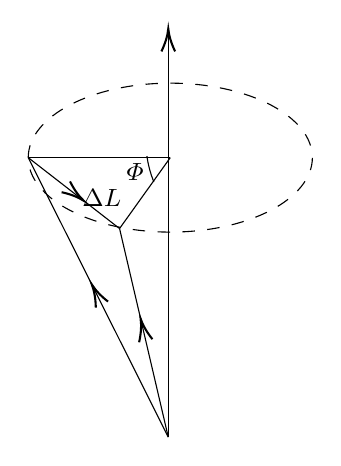
\begin{tikzpicture}[x=0.75pt,y=0.75pt,yscale=-1,xscale=1]
        %uncomment if require: \path (0,300); %set diagram left start at 0, and has height of 300

        %Shape: Ellipse [id:dp48022053498348405] 
        \draw  [dash pattern={on 4.5pt off 4.5pt}] (242.1,104.07) .. controls (242.1,84.26) and (272.75,68.19) .. (310.55,68.19) .. controls (348.35,68.19) and (379,84.26) .. (379,104.07) .. controls (379,123.88) and (348.35,139.95) .. (310.55,139.95) .. controls (272.75,139.95) and (242.1,123.88) .. (242.1,104.07) -- cycle ;
        %Straight Lines [id:da6368020376798296] 
        \draw    (242.1,104.07) -- (309.57,238.7) ;
        \draw [shift={(272.7,165.13)}, rotate = 63.38] [color={rgb, 255:red, 0; green, 0; blue, 0 }  ][line width=0.75]    (10.93,-3.29) .. controls (6.95,-1.4) and (3.31,-0.3) .. (0,0) .. controls (3.31,0.3) and (6.95,1.4) .. (10.93,3.29)   ;
        %Straight Lines [id:da6657087148655647] 
        \draw    (286.1,138.24) -- (309.57,238.7) ;
        \draw [shift={(296.24,181.66)}, rotate = 76.85] [color={rgb, 255:red, 0; green, 0; blue, 0 }  ][line width=0.75]    (10.93,-3.29) .. controls (6.95,-1.4) and (3.31,-0.3) .. (0,0) .. controls (3.31,0.3) and (6.95,1.4) .. (10.93,3.29)   ;
        %Straight Lines [id:da1380053955267717] 
        \draw    (242.1,104.07) -- (286.1,138.24) ;
        \draw [shift={(268.84,124.84)}, rotate = 217.83] [color={rgb, 255:red, 0; green, 0; blue, 0 }  ][line width=0.75]    (10.93,-3.29) .. controls (6.95,-1.4) and (3.31,-0.3) .. (0,0) .. controls (3.31,0.3) and (6.95,1.4) .. (10.93,3.29)   ;
        %Straight Lines [id:da9257959594233605] 
        \draw    (309.57,238.7) -- (309.57,43.96) ;
        \draw [shift={(309.57,41.96)}, rotate = 90] [color={rgb, 255:red, 0; green, 0; blue, 0 }  ][line width=0.75]    (10.93,-3.29) .. controls (6.95,-1.4) and (3.31,-0.3) .. (0,0) .. controls (3.31,0.3) and (6.95,1.4) .. (10.93,3.29)   ;
        %Straight Lines [id:da041606756368295805] 
        \draw    (242.1,104.07) -- (310.55,104.07) ;
        %Straight Lines [id:da02625225536450637] 
        \draw    (286.1,138.24) -- (310.55,104.07) ;
        %Shape: Arc [id:dp3586446455718637] 
        \draw  [draw opacity=0] (302.62,115.73) .. controls (300.95,111.68) and (299.85,107.52) .. (299.29,103.32) -- (357.53,96.74) -- cycle ; \draw   (302.62,115.73) .. controls (300.95,111.68) and (299.85,107.52) .. (299.29,103.32) ;



        % Text Node
        \draw (288.27,105.83) node [anchor=north west][inner sep=0.75pt]  [font=\small] [align=left] {$\displaystyle \varPhi $};
        % Text Node
        \draw (266.98,118.2) node [anchor=north west][inner sep=0.75pt]  [font=\small] [align=left] {$\displaystyle \Delta L$};


    \end{tikzpicture}
\end{center}

这里我们假设的角动量是和磁矩方向一致的,这样就导致了施加在磁矩上的力矩也能使得
角动量发生改变,而不是最后稳定在与B平行的位置,因此才有了进动现象。得到进动频率:
\begin{align*}
     & \tau =\frac{dL}{dt}=\mu \times B                                                     \\
     & \Delta L = \mu \times B \Delta t                                                     \\
     & L\sin \theta d\varPhi = \gamma L B \sin\theta \Delta t\Rightarrow\omega_0 = \gamma B
\end{align*}
注意这里的正负,如果$\omega_0$和B的方向相同则是正的,如果是相反的则是负的。
\section{The motion of charged particles in magnetic field}
\subsection{Fine Structure}
In quantum mechanics, 
we choose the coulomb gauge which satisfis the equation 
$\nabla \times A = B$ and $\nabla \dot A =0$, the Halmitonian of a 
single partical in magnetic field is:
\begin{align*}
    H=\frac{1}{2m}(P-qA/c)^2+V
\end{align*}
We choose the Landau gauge that satisfis the equation:
\begin{align*}
    A_x = -\frac{1}{2} yB\quad A_y = \frac{1}{2} xB
\end{align*}
Substitude these equtions,we obtain:
\begin{align*}
    H &= \frac{1}{2u}((P_x+\frac{qBy}{2c})^2+(P_y-\frac{qBx}{2c})+P_z^2)+V\\
    &= \frac{1}{2u}(P^2+\frac{q^2B^2}{4c^2}(x^2+y^2)-\frac{qBL_z}{c})+V
\end{align*}
Due to $B^2 \ll B$,Term $B^2$ can be neglected, the remaining term is
the interaction between magnetic field and orbital angular momentum:
\begin{align*}
    H_{interaction} = -\frac{qB}{2uc}L_z = -\mu_z B,\quad \mu_z = -\gamma L_z
\end{align*}
$\mu$ is orbital moment, we can quantize it from the above equations and obtain:
\begin{align*}
    \mu_z = \gamma L_z=\gamma m\hbar(n=0,\pm 1\cdots \pm l)
\end{align*}

When considering LS intheraction which gives rise to fine 
structure, the energy level will split. At this point,
\begin{align*}
    H = T+V+H_{LS}\\
    H_{LS} = \frac{1}{m^2_e c^2}\frac{1}{r}\dv{V_c}{r}(L\cdot S)
\end{align*}
\subsection{Zeeman effect}
塞曼效应是原子光谱在磁场中发生分裂的现象,当总自旋为0,对应正常塞曼效应,否则
对应反常塞曼效应,

\subsection{自旋相互作用随时间的演化}
根据第一章中提出的传播子的定义式:
\begin{align*}
    U(t)= \exp(\frac{-iHt}{\hbar})=\exp(\frac{i\gamma S_z B_k t}{\hbar})
\end{align*}
代入$H_{interaction}$可以得到:
\begin{align*}
      & U(t)=\exp (\frac{i\omega_0 \sigma_z t}{2})=\mqty[\cos {\omega_0t/2}+i\sin{\omega_0t/2} & 0 \\
    0 & \cos {\omega_0t/2}-i\sin{\omega_0t/2}]
\end{align*}
将传播子作用于任意方向的自旋本征态
\begin{align*}
    \begin{split}
        \ket{n+} &= \mqty[\cos{\frac{\theta}{2}}e^{-i\phi/2 } \\ \sin{\frac{\theta}{2}}e^{i\phi/2 }]
    \end{split}
    \quad &
    \begin{split}
        \ket{n-} &= \mqty[-\sin{\frac{\theta}{2}}e^{-i\phi/2 } \\ \cos{\frac{\theta}{2}}e^{i\phi/2} ]
    \end{split} \\
    \begin{split}
        \ket{\psi_+(t)} &= \mqty[\cos{\frac{\theta}{2}}e^{-i(\phi+\omega_0 t)/2 }\\\sin{\frac{\theta}{2}}e^{i(\phi-\omega_0t)/2 }]
    \end{split}
    \quad &
    \begin{split}
        \ket{\psi_-(t)} &= \mqty[-\sin{\frac{\theta}{2}}e^{-i(\phi+\omega_0 t)/2}\\\cos{\frac{\theta}{2}}e^{i(\phi-\omega_0t)/2 }]
    \end{split}
\end{align*}
\subsection{正常塞曼效应}
在强磁场下,能级发生分裂,并分裂成三条的现象叫做正常塞满效应,其中分裂成三条是由选择
定则决定的,结合7.1节得到的H($B^2 \ll B$):
\begin{align*}
    H = \frac{P^2}{2u}-\frac{e^2}{r}+\frac{eBL_z}{2uc}
\end{align*}
此时的能级为:
\begin{align*}
    E = E_{nlm}+\frac{eB\hbar}{2uc}m=E_{nlm}+\hbar \omega_L m\quad m = 0,\pm 1\cdots
\end{align*}
根据选择定则$\Delta m =\pm 1,0$,则能级分裂为三条。如果考虑到自旋磁矩与磁场的相互
作用:
\begin{align*}
    H = \frac{P^2}{2u}-\frac{e^2}{r}+\frac{eBL_z}{2uc}+\frac{eBS_z}{uc}
\end{align*}
这里还是选取$\ket{\bm{l^2},\bm{l_z}}$为本征态,得到此时的能级为:
\begin{align*}
    E = E_{nlm}+\hbar \omega_L (m\pm 1)
\end{align*}
可以看见加入自旋之后对能级分裂没有影响。
\subsection{反常塞曼效应}
除了$\bm{l}$和$\bm{s}$单独和磁场的作用,在磁场较弱时,$\bm{l}$和$\bm{s}$发生的相互作用不可
忽略,此时的哈密顿量:
\begin{align*}
    H = \frac{P^2}{2u}-\frac{e^2}{r}+\frac{eB}{2uc}(\bm{J_z}+\bm{S_z})+\varepsilon(r)\bm{l}\cdot \bm{s}
\end{align*}
$\bm{S_z}$和$\bm{S^2}$不是对易的,但是我们仍然可以选择$\ket{H,\bm{J^2},\bm{J_z},\bm{l^2},\bm{s^2}}$为本征态
而把$\bm{S_z}$视为微扰。根据微扰论,一阶能量近似:
\begin{align*}
    E^{1} = \bra{\bm{J^2},\bm{J_z},\bm{l^2},\bm{s^2}}\bm{S_z}\ket{\bm{J^2},\bm{J_z},\bm{l^2},\bm{s^2}}
\end{align*}
展开到$\ket{\bm{l_z},\bm{s_z},\bm{l^2},\bm{s^2}}$本征态上求平均值。
\begin{align*}
     & \left|j=l+\frac{1}{2}, m\right\rangle=\frac{1}{\sqrt{2l+1}}
    \left(\sqrt{l+\frac{1}{2}+m}\left|\left.l, m-\frac{1}{2}, \frac{1}{2}, \frac{1}{2}\right\rangle+
    \sqrt{l+\frac{1}{2}-m}\right| l, m+\frac{1}{2}, \frac{1}{2},-\frac{1}{2}\right\rangle \\
     & \ket{j=l-\frac{1}{2},m}=\frac{1}{\sqrt{21+1}}\left(-\sqrt{1+\frac{1}{2}-m}\ket{l,m-\frac{1}{2},\frac{1}{2},\frac{1}{2}}+\sqrt{l+\frac{1}{2}+m}
    \ket{l, m+\frac{1}{2}, \frac{1}{2},-\frac{1}{2}}\right)
\end{align*}
可以得到:
\begin{align*}
    E^1 = \begin{cases}
        &\frac{m}{2j+1}\quad j = l+\frac{1}{2}\\
        &\frac{-m}{2j+2} \quad j = l-\frac{1}{2}
    \end{cases}
\end{align*}
考虑到ls耦合之后,能级继续分裂成$\bm{l}+\frac{1}{2}$和$\bm{l}-\frac{1}{2}$两条
谱线,因此反常塞曼效应分裂的能级一般为偶数条。
\section{角动量}
\subsection{角动量耦合}
已知在$(J_1^2,J_2^2,J_{1z},J_{2z})$的本征态下,和自旋进行类比得到:
\begin{align*}
     & J_z \ket{j_1m_1,j_2m_2}=(J_{1z}+J_{2z})\ket{j_1m_1,j_2m_2}=(m_1+m_2)\hbar\ket{j_1m_1,j_2m_2} \\
     & J^2 \ket{j_1m_1,j_2m_2} = (J_1^2+J_2^2+2(J_+J_-+J_-J_++J_{1z}J_{2z}))\ket{j_1m_1,j_2m_2}
\end{align*}
假设:$\ket{j_1+j_2,j_1+j_2}=\ket{j_1j_1,j_2j_2}$,为了方便起见,我们在这里选取总自旋为0或者1
的态,利用阶梯算符(是总的还是分量需要对应好),我们现在用乘积右矢来表示总的右矢:
\begin{align*}
     & \ket{11}=\ket{++}                                                     \\
     & S_-\ket{11}=\sqrt{(j+m)(j-m+1)}\hbar \ket{10}=\sqrt{2}\hbar\ket{{10}} \\
     & (S_{1-}+S_{2-})\ket{++}=\hbar(\ket{+-}+\ket{-+})                      \\
     & \ket{10}=\frac{1}{\sqrt{2}}(\ket{+-}+\ket{-+})
\end{align*}
现在对于角动量问题:先说明一下简并性的问题:对于两个角动量的耦合,这里注意是角动量的
量子数,算符没有简并这一概念,例如对于$J=J_1+J_2$还是不变的,但是对于角动量量子数现在可以是:
$j_1+j_2,j_1+j_2-1,j_1+j_2-2\cdots j_1-j_2$,磁量子数:$m=\pm j$,因此简并度:
\begin{align*}
    \sum_{j_1-j_2}^{j_1+j_2} 2j+1 =(2j_1+1)(2j_2+1)
\end{align*}
这里有一个很方便的图表:
\begin{table}
    \centering
    \begin{tabular}{llll}
        \toprule
        $j_{1}+j_{2}$                                                & $j_{1}+j_{2}-1$                                                & $\cdots$ & $j_{1}-j_{2}$                                    \\
        \midrule
        $\left|j_{1}+j_{2}, j_{1}+j_{2}\right\rangle$                &                                                                &          &                                                  \\
        $\left|j_{1}+j_{2}, j_{1}+j_{2}-1\right\rangle$              & $\left|j_{1}+j_{2}-1, j_{1}+j_{2}-1\right\rangle$              &          &                                                  \\
        $\left|j_{1}+j_{2}, j_{1}+j_{2}-2\right\rangle$              & $\left|j_{1}+j_{2}-1, j_{1}+j_{2}-2\right\rangle$              &          & $\left|j_{1}-j_{2}, j_{1}-j_{2}\right\rangle$    \\
        $\cdots$                                                     & $\cdots$                                                       & $\cdots$ & $\cdots$                                         \\
        $\left|j_{1}+j_{2},-\left(j_{1}+j_{2}-2\right)\right\rangle$ & $\left|j_{1}+j_{2}-1,-\left(j_{1}+j_{2}-2\right)\right\rangle$ &          & $\left|j_{1}-j_{2}, -(j_{1}-j_{2})\right\rangle$ \\
        $\left|j_{1}+j_{2},-\left(j_{1}+j_{2}-1\right)\right\rangle$ & $\left|j_{1}+j_{2}-1,-\left(j_{1}+j_{2}-1\right)\right\rangle$ &          &                                                  \\
        $\left|j_{1}+j_{2},-\left(j_{1}+j_{2}\right)\right\rangle$   &                                                                &          &                                                  \\
        \bottomrule
    \end{tabular}
    \caption{角量子数}
    \label{tab:zeeman_table}
\end{table}

这里也举一个例子:对于第一列的最顶端的态,通过阶梯算符寻找底下的态与其关系:
\begin{align*}
     & \ket{j_1+j_2,j_1+j_2}=\ket{j_1j_1,j_2j_2}                                                                                                   \\
     & J_-\ket{j_1+j_2,j_1+j_2}=\sqrt{(j+m)(j-m+1)}\hbar\ket{j_1+j_2,j_1+j_2-1}=\sqrt{2(j_1+j_2)}\hbar\ket{j_1+j_2,j_1+j_2-1}                      \\
     & (J_{1-}+J_{1+})\ket{j_1j_1,j_2j_2}=\sqrt{(2j_1)}\hbar \ket{j_1(j_1-1),j_2j_2}+\sqrt{2j_2}\hbar \ket{j_1j_1,j_2(j_2-1)}                      \\
     & \ket{j_1+j_2,j_1+j_2-1}=(\frac{j_1}{j_1+j_2})^{\frac{1}{2}}\ket{j_1(j_1-1),j_2j_2}+(\frac{j_2}{j_1+j_2})^\frac{1}{2}\ket{j_1j_1,j_2(j_2-1)}
\end{align*}
按这样的方法从上往下计算,就可以得到下面所有的态与非耦合态矢的关系,对于第二列的第一个我们
采用这样的一个习惯:
\begin{align*}
    \ket{j_1+j_2-1,j_1+j_2-1}=a\ket{j_1(j_1-1),j_2j_2}+b\ket{j_1j_1,j_2(j_2-1)}
\end{align*}
需要满足正交归一性:
\begin{align*}
    \begin{cases}
        a^2+b^2=1 \\
        a(\frac{j_1}{j_1+j_2})^{\frac{1}{2}}+b(\frac{j_2}{j_1+j_2})^\frac{1}{2}=0
    \end{cases}
    \Rightarrow \begin{cases}
                    a=-(\frac{j_2}{j_1+j_2})^\frac{1}{2} \\
                    b=(\frac{j_1}{j_1+j_2})^{\frac{1}{2}}
                \end{cases}
\end{align*}
这样继续重复第一列第一行的步骤,就可以得到下面所有的态与非耦合态矢的关系,后面的列以此类推。
由上面的步骤,我们还可以引入CG系数:
\begin{align*}
    \ket{jm,j_1j_2}=\sum_{m_1,m_2}\ket{j_1m_1,j_2m_2}\braket{j_1m_1,j_2m_2}{jm,j_1j_2}
\end{align*}
\section{近似方法}
\subsection{不含时非简并微扰理论}
当哈密顿量写成$H=H^0+H^1$时,$H^0$时非微扰哈密顿量,$H^1$是微扰哈密顿量,
微扰哈密顿量相对于非微扰哈密顿量是非常小的,可以看成是很弱的外场的作用引起
的,具体的数学过程如下:
\begin{align*}
     & (H^0+H^1)(\ket{n^0}+\ket{n^1}+\ket{n^2}+\cdots)=(E_n^0+E_n^1+E_n^2+E_n^3+\cdots)
    (\ket{n^0}+\ket{n^1}+\ket{n^2}+\cdots)                                              \\&H^0\ket{n^0}=E_n^0\ket{n^0}
    \text{(zero order)}                                                                 \\&H^0\ket{n^1}+H^1\ket{n^0}=E_n^0\ket{n^1}+E_n^1\ket{n^0}\text
    {(first order)}                                                                     \\&H^0\ket{n^2}+H^1\ket{n^1}+H^2\ket{n^0}=E_n^0\ket{n^2}+E_n^1\ket{n^1}
    +E_n^2\ket{n^0}\text{(second order)}
\end{align*}
可以利用上面的公式求得能量一级二级近似,以及态矢以及修正:
\begin{align*}
     & \mel{n^0}{H^0}{n^1}+\mel{n^0}{H^1}{n^0}=E_n^1\braket{n^0}{n^0}+E_n^0\braket{n^0}{n^1}
    \Rightarrow E_n^1=\mel{n^0}{H^1}{n^0}                                                    \\
     & \mel{m^0}{H^0}{n^1}+\mel{m^0}{H^1}{n^0}=E_n^1\braket{m^0}{n^0}+E_n^0\braket{m^0}{n^1} \\
     & \Rightarrow E_m^0\braket{m^0}{n^1}+\mel{m^0}{H^1}{n^0}=E_n^0\braket{m^0}{n^0}         \\
     & \Rightarrow \braket{m^0}{n^1}=\frac{\mel{m^0}{H^1}{n^0}}{E_n^0-E_m^0}
\end{align*}
上面求出来了$\ket{n^1}$在$\ket{m^0}$上的投影,现在我们寻找$\ket{n^1}$在$\ket{n^0}$上的投影,这样两者加
起来就是态矢的一级修正了,或者插入一个封闭关系得到:
\begin{tcolorbox}[colframe=red]
    $$\ket{n^1}=\sum_m \ket{m^0}\frac{\mel{m^0}{H^1}{n^0}}{E_n^0-E_m^0}$$
\end{tcolorbox}

能量二阶修正:
\begin{align*}
    \text{left product} \bra{n^0}\Rightarrow E_n^2=\mel{n^0}{H^1}{n^1}
\end{align*}
更高级的近似依次类推。
\subsection{简并微扰}
当出现$E_n^0=E_m^0$时,上述的非简并微扰方法需要做出一定的修正,才可以继续被使用
首先先从最方便的二重简并开始讨论:
\begin{align*}
    H\ket{E}=E\ket{E}(\ket{E}=\alpha\ket{E_a}+\beta\ket{E_b})
\end{align*}
这里简并子空间是二维的,由于微扰的结果是消除了简并,这里考虑到$H^0$有一个简并的子空间,$H^0+H^1$在
这个空间中是非简并的,是我们可以将两个简并的态矢带入到前面的一阶近似方程里面:
\begin{align*}
     & H^0\ket{n^1}+H^1(\alpha\ket{E_a^0}+\beta\ket{E_b^0})=E_n^0\ket{n^1}+E_n^1
    (\alpha\ket{E_a^0}+\beta\ket{E_b^0})
\end{align*}
product $\ket{\psi_a}$ on both sides of the equation:
\begin{align*}
     & \alpha\mel{E_a}{H^1}{E_a}+\beta\mel{E_a}{H^1}{E_b}=\alpha E_n^1            \\
     & \alpha\mel{E_b}{H^1}{E_b}+\beta\mel{E_b}{H^1}{E_b}=\beta E_n^1             \\
     & \mqty(H_{aa}^1                                                  & H_{ab}^1 \\H_{bb}^1&H_{ba}^1)\mqty(\alpha\\ \beta)=E_n^1\mqty
    (\alpha                                                                       \\\beta)
\end{align*}
得到的能量本征值为对应本征态的一阶修正

\begin{tcolorbox}[colframe=red!75!]
非简并态微扰公式失效的原因是在一阶能量修正以及更高阶
的部分,分母为0,根据极限定义,可以令$H^1$的非对角元为0即可,也就是所谓的对角化,
只需要在简并空间当中选择一组合适的基,这组合适的基能够使得$H^1$对角化,选择了合适的基之后,之前
失效的公式现在又成立了,因此对角元就是对应的能量的一级修正。
\end{tcolorbox}


如果求得的一阶能量近似仍然是简并的,可以利用二阶近似公式,通过代入简并态的线性组合
构成一个新的矩阵方程,来使零级波函数的简并态进行分离。

\subsection{Degenerate pertubation problem}
notation: $\ket{n^{(0)},k}$ denotes 0-level approximation and k-level degeneracy of ket n.
We can use the following equtions to get some correction state and energy:
\begin{align*}
    \left\{\begin{array}{l}
    \left(H^0-E_{n k}^{(0)}\left|n^{(0)}, k\right\rangle=0 \right. \\
    \left(H^0-E_{n k}^{(0)}\right)\left|n^{(1)}, k\right\rangle=\left(E_{n k}^{(1)}-\delta H\right)\left|n^{(0)}, k\right\rangle \\
    \left(H^0-E_{n k}^{(0)}\right)\left|n^{(2)}, k\right\rangle=\left(E_{n k}^{(1)}-\delta H\right)\left|n^{(1)}, k\right\rangle+E_{n k}^{(2)}\left|n^{(0)}, k\right\rangle
    \end{array}\right.
\end{align*}
Due to $\ket{n^{(1)},k}$ and $\ket{n^{(0)},k}$ are not parallel. We define
the degenerate space $V_N = Span\{\ket{n^{(0)},k},k=0,1,2\cdots\}$. The
whole Helbert space $\mathcal{H} =V \oplus V_N$,
\begin{align*}
    (E_{nl}^{(0)}-E_{nk}^{(0)})\braket{n^{(0)},l}{n^{(1)},k} = E_{nk}^{(1)}
    \delta _{kl}-\bra{n^{(0)},l}\delta H \ket{n^{(0)},k}
\end{align*}
这两个能量是一样的,则可以得到能量的一阶修正:
\begin{align*}
    E_{nk}^{(1)}\delta_{kl} = \bra{n^{(0)},l}\delta H\ket{n^{(0)},k}
\end{align*}
现在考虑简并态矢的一阶修正

\subsection{Time dependent pertubation theorem} 

\begin{figure}[htbp]
\centering
\tikzset{every picture/.style={line width=0.75pt}} %set default line width to 0.75pt        
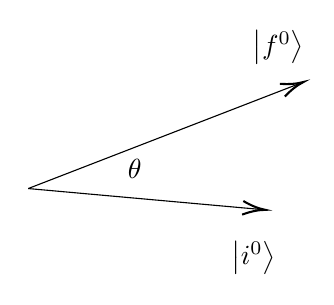
\begin{tikzpicture}[x=0.75pt,y=0.75pt,yscale=-1,xscale=1]
%uncomment if require: \path (0,300); %set diagram left start at 0, and has height of 300

%Straight Lines [id:da15634307517009205] 
\draw    (219.2,194.92) -- (331.44,205.01) ;
\draw [shift={(333.43,205.18)}, rotate = 185.14] [color={rgb, 255:red, 0; green, 0; blue, 0 }  ][line width=0.75]    (10.93,-3.29) .. controls (6.95,-1.4) and (3.31,-0.3) .. (0,0) .. controls (3.31,0.3) and (6.95,1.4) .. (10.93,3.29)   ;
%Straight Lines [id:da12214970648848089] 
\draw    (219.2,194.92) -- (349.99,144.3) ;
\draw [shift={(351.85,143.57)}, rotate = 158.84] [color={rgb, 255:red, 0; green, 0; blue, 0 }  ][line width=0.75]    (10.93,-3.29) .. controls (6.95,-1.4) and (3.31,-0.3) .. (0,0) .. controls (3.31,0.3) and (6.95,1.4) .. (10.93,3.29)   ;


% Text Node
\draw (315.97,218.99) node [anchor=north west][inner sep=0.75pt]    {$\ket{i^{0}}$};
% Text Node
\draw (326.14,117.68) node [anchor=north west][inner sep=0.75pt]    {$\ket{f^{0}}$};
% Text Node
\draw (266,179.4) node [anchor=north west][inner sep=0.75pt]    {$\theta $};
\end{tikzpicture} 
\caption{the time evolution of ket}
\label{fig:evolution}
\end{figure}                
After time t,$\ket{i^0}\rightarrow \ket{f^0}$的跃迁概率是多少,跃迁概率
是远远小于1的,推导过程:
\begin{align*}
    \ket{\psi }=\sum_n d_n(t)\ket{n^0}e^{-iE_n^{0} t/hbar}
\end{align*}
Substituting the above equation into the Schrödinger equation:
\begin{align*}
    i\hbar(\pdv{}{t}-H^0-H^1)\ket{\psi} & =\sum_n i\hbar (\pdv{}{t}-H^0-H^1)e^{-iE_n^0t/\hbar}d_n(t)\ket{n^0}
    \\\Rightarrow 0&=\sum_n [i\hbar\dot{d}_n(t)-H^1(t)d_n(t)]e^{-iE_n^0 t/\hbar}\ket{n^0}
\end{align*}
multiply  $\bra{f^0}e^{-iE_f^0t/\hbar}$both sides of the equation:
\begin{align*}
    i\hbar \dot{d}_f(t)=\sum_n \mel{f^0}{H^1}{n^0}e^{-i\omega_ft/\hbar}d_n(t)
\end{align*}
对于0级近似, $H^{1} = 0$,态矢处于能量本征态$\ket{i^0}$,
\begin{align*}
    d_n(0) = \delta_{ni}
\end{align*}
for 1-th order approximation, we substitude 0-th order approximation into
time evolution equation.
\begin{align*}
    i\hbar \dot{d}_f(t)=\sum_n \mel{f^0}{H^1}{n^0}e^{-i\omega_ft/\hbar}\delta _{ni}
\end{align*}
for n-th order approximation:
\begin{align*}
    i\hbar \dot{d}_f(t)=\sum_n \mel{f^0}{H^1}{n^0}e^{-i\omega_ft/\hbar}d_n(t)
\end{align*}


\newpage
\subsection{Calculus of variations}
Next,we will provide energy funtional and find its extremum,
let$Q=\braket{\psi}{\psi},P=\mel{\psi}{H}{\psi}$ and $E[\psi]=P/Q$.
\begin{align*}
    \delta E & = \frac{\mel{\psi+\delta \psi}{H}{\psi +\delta \psi}}{\braket{\psi+\delta\psi}{\psi+\delta\psi}}
    -\frac{\mel{\psi}{H}{\psi}}{\braket{\psi}{\psi}}                                                                           \\
             & \approx \frac{Q(\mel{\psi}{H}{\psi}+\mel{\psi}{H}{\delta\psi}+\mel{\delta\psi}{H}{\psi})-(Q+\braket{\delta\psi}
        {\psi}+\braket{\psi}{\delta \psi})\mel{\psi}{H}{\psi}}{(Q+\braket{\delta\psi}
    {\psi}+\braket{\psi}{\delta \psi})Q}                                                                                       \\
             & =\frac{\mel{\psi}{H}{\delta\psi}+\mel{\delta\psi}{H}{\psi}-(\braket{\delta\psi}
        {\psi}+\braket{\psi}{\delta \psi})P/Q}{Q+\braket{\delta\psi}
        {\psi}+\braket{\psi}{\delta \psi}}
\end{align*}
Therefore, We can derive from above fomular when $\delta E=0$:
\begin{align*}
    H\ket{\psi}=E\ket{\psi}
\end{align*}
Choose a set of basis:$\ket{\psi}=\sum_p C_p\ket{\chi_p}$:
\begin{align*}
     & \sum_{pq}C_pC_q^* \mel{\chi_q}{H}{\chi_p}=E\sum_{pq}C_pC_q^*\braket{\chi_q}{\chi_p}
    \\&E=\frac{\sum_{pq}C_pC_q^* \mel{\chi_q}{H}{\chi_p}}{\sum_{pq}C_pC_q^*\braket{\chi_q}{\chi_p}}
\end{align*}
Obtain the matrix form of stationary equation from above equation:
\begin{align*}
    (H_{pq}-E\delta_{pq})C_q=0
\end{align*}
The fundamental approach is to choose a set of basis which closely resemble 
the true ground state from Helbert space. Then, Solve the   matrix equation,
We can obtain the approximate ground state energy.

A poor approximation to the actual wave function can yield an excellent 
approximation to the real actual energy. The reason is following:
\begin{align*}
    (\bra{\phi}+\bra{\delta \phi_{\parallel}}+\bra{\delta \phi_{\bot}})H(\ket{\phi}
    +\ket{\delta \phi_{\parallel}}+\ket{\delta \phi_{\bot}})=|1+\alpha|^2 E+O(\delta\phi^2_{\bot})
    \quad (\ket{\phi_{\parallel}}=\alpha ,\ket{\delta \phi} \alpha\ll 1)
\end{align*}

In general, We can choose some vectors which are parametried 
by some variables $(\alpha,\beta,\cdots,\gamma)$ in Helbert space and 
which have the general features one expects of the true ground state
ket. The question becomes as following:
\begin{align*}
    E_0 \approx E(\alpha)_{min}
\end{align*}
\end{document}